\documentclass[a4paper, 11pt]{article}
\usepackage{geometry}
\geometry{letterpaper, margin=1in}
\usepackage{amsmath}
\usepackage{amssymb}  
\usepackage{amsthm}
\usepackage{ulem} 
\usepackage{graphicx}
\usepackage{enumitem} 
\graphicspath{ {images/} }


\newtheorem*{theorem}{Theorem}
\newtheorem*{corollary}{Corollary}
\newtheorem*{lemma}{Lemma}
\newtheorem*{definition}{Definition}
\newtheorem*{proposition}{Proposition}

\begin{document}
%Header-Make sure you update this information!!!!
\noindent
\large\textbf{Abstract Surfaces} \hfill \textbf{John Waczak} \\
\normalsize MTH 435 \hfill  Date: \today \\


	
	
\subsection*{Recap} 
	Goal: Free ourselves from $\mathbb{R}^3$. So far all of our surfaces were sitting in $\mathbb{R}^3$ i.e. $S\subseteq\mathbb{R}^3$. We also defined the tangent space for all points $p\in S$ as $T_p S$. Then we developed the differential geometry around a point p as a study of $T_p S$. \\ 
	
	\noindent We have seen that all notions of \textit{intrinsic geometry} such as $K$ the Gaussian curvature, geodesics, intrinsic distance, completeness, etc... were all defined in terms of the first fundamental form $\mathbb{I}$. The first fundamental form was really just a \textit{choice} of an inner product on each $T_p S$. 

\subsection*{Abstractions} 
	We want to define $S$ surfaces abstractly without any reference to $\mathbb{R}^3$ such that differentiable sets on S make sense and we can extend the intrinsic geometry to such sets. \\ 
	
	\textbf{This was very, very difficult to develop} \\ 

	\begin{definition}
		An \textit{Abstract Surface} (a.k.a differentiable, smooth $2-$manifold) is a set $S$ together with a family of injective maps (continuous) $x_\alpha:U_\alpha \to S$ of open sets $U_\alpha \subseteq \mathbb{R}^2$  (i.e. \textbf{Surface Charts}) into S such that 
			\begin{enumerate}
				\item $\cup_\alpha x_\alpha(U_\alpha) = S$ \\
				\item For each $\alpha, \beta$ with $x_\alpha(U_\alpha)\cap x_\beta(U_\beta) = W \neq \emptyset$. We have that $x_\alpha^{-1}(W)$, $x_\beta^{-1}(W)$ are open subsets of $\mathbb{R}^2$ and $x_\beta^{-1}\circ x_\alpha$, $x_\alpha^{-1}\circ x_\beta$ are differentiable. $W = x_\alpha(u_\alpha)\cap x_\beta(U_\beta)$. 
			\end{enumerate}
		\begin{figure}[!hbt]
			\centering
			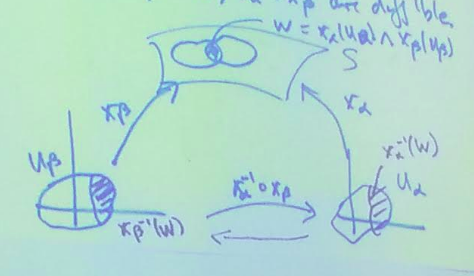
\includegraphics[width=0.65\columnwidth]{abstractDefinition}
			\caption{Pictorial representation of (2)}
		\end{figure}
		
		\noindent $(u_\alpha, x_\alpha)$ with $p\in x_\alpha(U_\alpha)$: parameterization or a coordinate chart of S around p. $q = x_\alpha(u_\alpha, v_\alpha)$ is how you map the point $(u_\alpha, v_\alpha)\in \mathbb{R}^2$ to the surface S. I.e. those arguments are the coordinates.\\ 
	
	\end{definition}
	
	
	\begin{definition}
		A \textit{differentiable structure} for S is a family $\{(U_\alpha, x_\alpha)\}$
	\end{definition}
	
	
	
	\noindent From (2) we have that a change of parameters $x_\beta^{-1}\circ x_\alpha : x_\alpha^{-1}(W)\to x_\beta^{-1}(W)$ is a diffeomorphism. \\
	
	\textbf{NOTE} Sometimes it is convenient to have further conditions  (differs from book to book). 
		\begin{enumerate}
			\item Differentiable structure $\{(U_\alpha, x_\alpha)\}$ should be maximal relative to conditions (1) and (2) above. ie.e any of the family satisfy (1) and (2) is already contained in $\{(U_\alpha, x_\alpha)\}$
			\item We may want Haussdorff, second countable $\rightarrow$ topology.
		\end{enumerate}
	\noindent These are conditions we use to define higher dimensional manifolds. 
	
	
	When we compare this to the old definition, the big difference is that (2) condition. 
	
	
\subsection*{What is a differentiable map?} 
	\textit{Remember:} we do not have $\mathbb{R}^3$ at our fingertips so we need to be precise. \\ 
	
	\begin{definition}
		If we have $S_1, S_2$ abstract surfaces and $\phi:S_1\to S_2$ is \textit{Differentiable} at $p\in S_1$ if given a parametrization $y:V\subset\mathbb{R}^2\to S_2$ around $\phi(p)$ $\exists$ a parametrization $x:U\subset\mathbb{R}^2\to S_1$ around p such that $\phi(x(U))\subset y(V)$ we want the image it land in $y$. And the map $y^{-1}\circ \phi \circ x:U\to \mathbb{R}^2$ is differentiable at $x^{-1}(p)$. We say $\phi$ is differentiable on $S_1$ if $\phi$ is differentiable for all p $\in S_1$. 
			\begin{figure}[!hbt]
				\centering
				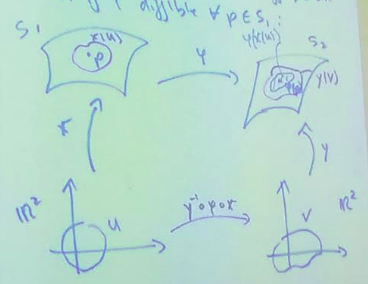
\includegraphics[width=0.65\columnwidth]{differentiable}
			\end{figure}
			
		\noindent\textbf{NOTE:} By condition (2) this does not depend on choice of parametrization. $y^{-1}\circ\phi\circ x$ is the expression of $\phi$ in the parametrizations x and y. 
	\end{definition}
	
	
	
	
\subsection*{Example: Real Projective Plane}	
	Let $S^2 = \{(x,y,z)\in \mathbb{R}^3 : x^2+y^2+z^2=1\}$ and define 
		\begin{align*}
			A:S^2&\to S^2 \quad \text{antipodal map} \\ 
			(x,y,z)&\to (-x,-y,-z) 
		\end{align*}
	Define $\mathbb{R}P^2 = \frac{S^2}{N}$ where $p\cong q$ for $p,q \in S^2$ iff $q = A(p)$. This means we get a map (the natural projection)
		\begin{align*}
			\pi:S^2 &\to \mathbb{R}P^2 \\ 
			p&\mapsto [p] = \{p, A(p)\}
		\end{align*} 
	
	\noindent Is this an abstract surface? \\ 
	
	\noindent Cover $S^2$ with coordinate charts $x_\alpha:U_\alpha\to S^2$ such that $x_\alpha(U_\alpha)\cap A\circ x_\alpha(U_\alpha) = \emptyset$  \\ 
	
	\noindent Now: $S^2$ is a regular surface, A is a diffeomorphism $\Rightarrow$ $\mathbb{R}P^2$ with $\{U_\alpha, \pi\circ x_\alpha\}$ is an abstract surface. We need to check that $\pi\circ x_\alpha$ is injective. \\ 
	
	\noindent Injectivity:
		\begin{align*}
			\pi(x_\alpha(x)) &= \pi(x_\alpha(y)) \\
			 \Rightarrow [x_\alpha(x)] &= [x_\alpha(y)] \\
			 \Rightarrow x_\alpha(x) &= x_\alpha(y) \text{ or } A(x_\alpha(y))
		\end{align*} 
		but $A(x_\alpha(y))$ is not in $x_\alpha(U_\alpha)$ $\rightarrow x_\alpha(x) = x_\alpha(y)$ which implies $x = y$ since $x_\alpha$ was injective already. 
	
	\begin{figure}[!hbt]
		\centering 
		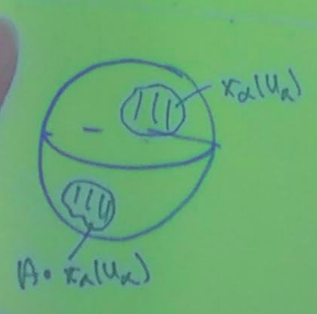
\includegraphics[width=0.5\columnwidth]{antipodal}
	\end{figure}
\end{document}






































